\documentclass[11pt]{article}
\usepackage{house}
\hypersetup{pdftitle={Do Price Signals Predict Indian Stock Returns? A Next-Day Forecast, a Monthly Strategy and a Survivorship-Free Test}, pdfauthor={Arjun Prashanth}, pdfkeywords={technical analysis, moving averages, momentum, survivorship bias, backtesting, India}}
% Generated by paper/make_assets.py. Do not edit by hand.
\newcommand{\NUniverse}{100}
\newcommand{\NStocks}{98}
\newcommand{\NExcluded}{2}
\newcommand{\NFull}{77}
\newcommand{\NPartial}{21}
\newcommand{\MeanTestDays}{345.4}
\newcommand{\MinTestDays}{225}
\newcommand{\MaxTestDays}{347}
\newcommand{\MedianObs}{1{,}731}
\newcommand{\MedianTrainObs}{1{,}384}
\newcommand{\RsqMean}{\ensuremath{-0.0155}}
\newcommand{\RsqMedian}{\ensuremath{-0.0090}}
\newcommand{\RsqMin}{\ensuremath{-0.130}}
\newcommand{\RsqMax}{\ensuremath{+0.042}}
\newcommand{\NRsqPos}{17}
\newcommand{\NRsqNeg}{81}
\newcommand{\AccMean}{49.6\%}
\newcommand{\AccSD}{3.1}
\newcommand{\AccMin}{41.3\%}
\newcommand{\AccMax}{55.3\%}
\newcommand{\AccTstat}{\ensuremath{-1.20}}
\newcommand{\UpMean}{47.8\%}
\newcommand{\EdgeMean}{\ensuremath{+1.85}}
\newcommand{\NEdgePos}{68}
\newcommand{\RandomEdge}{\ensuremath{+2.22}}
\newcommand{\NWeakBench}{73}
\newcommand{\EdgeBenchCorr}{0.55}
\newcommand{\NBeatRandom}{48}
\newcommand{\MedianTestChange}{\ensuremath{-0.06}\%}
\newcommand{\NRose}{49}
\newcommand{\SEAcc}{2.7}
\newcommand{\TwoSE}{5.4}
\newcommand{\MDEAcc}{57.5\%}
\newcommand{\MDEpp}{7.5}
\newcommand{\PooledSE}{0.31}
\newcommand{\NOutsideBand}{16}
\newcommand{\NAboveBand}{15}
\newcommand{\NBelowBand}{1}
\newcommand{\NSigAbove}{0}
\newcommand{\NSigBelow}{7}
\newcommand{\NSigAboveBH}{0}
\newcommand{\NSigBelowBH}{0}
\newcommand{\ExpectedPerTail}{2.5}
\newcommand{\NPTDefined}{97}
\newcommand{\NPTUndefined}{1}
\newcommand{\NPTSigPos}{5}
\newcommand{\NPTSigNeg}{0}
\newcommand{\NPTBH}{0}
\newcommand{\PTMedian}{0.37}
\newcommand{\PxMedian}{61.8\%}
\newcommand{\TopMaFive}{58}
\newcommand{\TopMaTwenty}{38}
\newcommand{\TopRet}{2}
\newcommand{\TopRatio}{0}
\newcommand{\NRatioPos}{61}
\newcommand{\NRatioNeg}{37}
\newcommand{\SignTestP}{0.02}
\newcommand{\RatioAbsMean}{0.0016}
\newcommand{\RatioAbsMeanPP}{0.16}
\newcommand{\RelTrainStart}{1~July~2019}
\newcommand{\RelTrainEnd}{31~January~2025}
\newcommand{\RelTestStart}{1~February~2025}
\newcommand{\RelTestEnd}{26~June~2026}
\newcommand{\RelTestDays}{347}
\newcommand{\RelPriceRsq}{0.936}
\newcommand{\RelNaiveRsq}{0.963}
\newcommand{\RelMAEcut}{27\%}
\newcommand{\RelActLo}{\ensuremath{-4.6}\%}
\newcommand{\RelActHi}{\ensuremath{+5.3}\%}
\newcommand{\RelPredBand}{0.47\%}
\newcommand{\RelCloseSD}{93.9}
\newcommand{\RelRWRMSE}{18.1}
\newcommand{\RelPriceDir}{47.0\%}
\newcommand{\RelNaiveDir}{51.6\%}
\newcommand{\RelReturnDir}{51.0\%}
\newcommand{\RelUpShare}{48.4\%}
\newcommand{\RelEdge}{\ensuremath{+2.6}}
\newcommand{\CrossGolden}{28~August~2019}
\newcommand{\CrossDeath}{8~November~2019}
\newcommand{\MedianFullGrowth}{2.73}
\newcommand{\MeanAbsMaFive}{128.1}
\newcommand{\MeanAbsMaTwenty}{126.5}
\newcommand{\MeanAbsRatioBp}{16.2}
\newcommand{\SurvCagrDev}{31.0\%}
\newcommand{\SurvEwCagrDev}{26.9\%}
\newcommand{\SurvNiftyCagrDev}{16.1\%}
\newcommand{\SurvSharpeDev}{1.14}
\newcommand{\SurvEwSharpeDev}{0.81}
\newcommand{\SurvNiftySharpeDev}{0.50}
\newcommand{\SurvMaxDDDev}{\ensuremath{-27.9}\%}
\newcommand{\SurvEwMaxDDDev}{\ensuremath{-32.9}\%}
\newcommand{\SurvActiveDev}{\ensuremath{+2.4}\%}
\newcommand{\SurvActiveTDev}{0.47}
\newcommand{\SurvAlphaDev}{\ensuremath{+8.5}\%}
\newcommand{\SurvAlphaTDev}{2.73}
\newcommand{\SurvDsrDev}{0.99}
\newcommand{\SurvCostDev}{2.6\%}
\newcommand{\SurvTurnoverDev}{405\%}
\newcommand{\SurvBreakEvenDev}{2.1}
\newcommand{\SurvNamesDev}{55}
\newcommand{\SurvSharpeLoDev}{0.46}
\newcommand{\SurvSharpeHiDev}{1.85}
\newcommand{\SurvCagrHold}{33.3\%}
\newcommand{\SurvEwCagrHold}{22.7\%}
\newcommand{\SurvNiftyCagrHold}{13.0\%}
\newcommand{\SurvSharpeHold}{1.16}
\newcommand{\SurvEwSharpeHold}{0.80}
\newcommand{\SurvNiftySharpeHold}{0.48}
\newcommand{\SurvMaxDDHold}{\ensuremath{-36.9}\%}
\newcommand{\SurvEwMaxDDHold}{\ensuremath{-39.7}\%}
\newcommand{\SurvActiveHold}{\ensuremath{+8.5}\%}
\newcommand{\SurvActiveTHold}{2.67}
\newcommand{\SurvAlphaHold}{\ensuremath{+9.9}\%}
\newcommand{\SurvAlphaTHold}{3.19}
\newcommand{\SurvDsrHold}{0.95}
\newcommand{\SurvCostHold}{2.5\%}
\newcommand{\SurvTurnoverHold}{396\%}
\newcommand{\SurvBreakEvenHold}{5.2}
\newcommand{\SurvNamesHold}{55}
\newcommand{\SurvSharpeLoHold}{0.41}
\newcommand{\SurvSharpeHiHold}{2.13}
\newcommand{\SurvCagrFull}{32.0\%}
\newcommand{\SurvEwCagrFull}{25.0\%}
\newcommand{\SurvNiftyCagrFull}{14.8\%}
\newcommand{\SurvSharpeFull}{1.15}
\newcommand{\SurvEwSharpeFull}{0.81}
\newcommand{\SurvNiftySharpeFull}{0.50}
\newcommand{\SurvMaxDDFull}{\ensuremath{-36.9}\%}
\newcommand{\SurvEwMaxDDFull}{\ensuremath{-45.5}\%}
\newcommand{\SurvActiveFull}{\ensuremath{+5.0}\%}
\newcommand{\SurvActiveTFull}{1.60}
\newcommand{\SurvAlphaFull}{\ensuremath{+9.2}\%}
\newcommand{\SurvAlphaTFull}{4.09}
\newcommand{\SurvDsrFull}{1.00}
\newcommand{\SurvCostFull}{2.5\%}
\newcommand{\SurvTurnoverFull}{401\%}
\newcommand{\SurvBreakEvenFull}{3.4}
\newcommand{\SurvNamesFull}{55}
\newcommand{\SurvSharpeLoFull}{0.60}
\newcommand{\SurvSharpeHiFull}{1.73}
\newcommand{\PitCagrDev}{21.3\%}
\newcommand{\PitEwCagrDev}{16.4\%}
\newcommand{\PitNiftyCagrDev}{17.4\%}
\newcommand{\PitSharpeDev}{0.69}
\newcommand{\PitEwSharpeDev}{0.43}
\newcommand{\PitNiftySharpeDev}{0.56}
\newcommand{\PitMaxDDDev}{\ensuremath{-34.7}\%}
\newcommand{\PitEwMaxDDDev}{\ensuremath{-49.3}\%}
\newcommand{\PitActiveDev}{\ensuremath{+2.8}\%}
\newcommand{\PitActiveTDev}{0.48}
\newcommand{\PitAlphaDev}{\ensuremath{+6.9}\%}
\newcommand{\PitAlphaTDev}{2.12}
\newcommand{\PitDsrDev}{0.85}
\newcommand{\PitCostDev}{2.7\%}
\newcommand{\PitTurnoverDev}{418\%}
\newcommand{\PitBreakEvenDev}{2.4}
\newcommand{\PitNamesDev}{80}
\newcommand{\PitSharpeLoDev}{0.07}
\newcommand{\PitSharpeHiDev}{1.34}
\newcommand{\PitMomCagrDev}{23.6\%}
\newcommand{\PitMomSharpeDev}{0.86}
\newcommand{\PitMomMaxDDDev}{\ensuremath{-28.3}\%}
\newcommand{\PitCagrHold}{27.3\%}
\newcommand{\PitEwCagrHold}{17.3\%}
\newcommand{\PitNiftyCagrHold}{14.2\%}
\newcommand{\PitSharpeHold}{0.93}
\newcommand{\PitEwSharpeHold}{0.58}
\newcommand{\PitNiftySharpeHold}{0.54}
\newcommand{\PitMaxDDHold}{\ensuremath{-37.0}\%}
\newcommand{\PitEwMaxDDHold}{\ensuremath{-45.8}\%}
\newcommand{\PitActiveHold}{\ensuremath{+8.3}\%}
\newcommand{\PitActiveTHold}{2.39}
\newcommand{\PitAlphaHold}{\ensuremath{+9.6}\%}
\newcommand{\PitAlphaTHold}{2.64}
\newcommand{\PitDsrHold}{0.89}
\newcommand{\PitCostHold}{2.6\%}
\newcommand{\PitTurnoverHold}{416\%}
\newcommand{\PitBreakEvenHold}{5.1}
\newcommand{\PitNamesHold}{80}
\newcommand{\PitSharpeLoHold}{0.21}
\newcommand{\PitSharpeHiHold}{1.84}
\newcommand{\PitMomCagrHold}{19.7\%}
\newcommand{\PitMomSharpeHold}{0.71}
\newcommand{\PitMomMaxDDHold}{\ensuremath{-36.8}\%}
\newcommand{\PitCagrFull}{23.8\%}
\newcommand{\PitEwCagrFull}{16.8\%}
\newcommand{\PitNiftyCagrFull}{16.0\%}
\newcommand{\PitSharpeFull}{0.80}
\newcommand{\PitEwSharpeFull}{0.48}
\newcommand{\PitNiftySharpeFull}{0.55}
\newcommand{\PitMaxDDFull}{\ensuremath{-37.0}\%}
\newcommand{\PitEwMaxDDFull}{\ensuremath{-58.1}\%}
\newcommand{\PitActiveFull}{\ensuremath{+5.2}\%}
\newcommand{\PitActiveTFull}{1.43}
\newcommand{\PitAlphaFull}{\ensuremath{+8.4}\%}
\newcommand{\PitAlphaTFull}{3.46}
\newcommand{\PitDsrFull}{0.95}
\newcommand{\PitCostFull}{2.6\%}
\newcommand{\PitTurnoverFull}{417\%}
\newcommand{\PitBreakEvenFull}{3.6}
\newcommand{\PitNamesFull}{80}
\newcommand{\PitSharpeLoFull}{0.29}
\newcommand{\PitSharpeHiFull}{1.34}
\newcommand{\PitMomCagrFull}{21.9\%}
\newcommand{\PitMomSharpeFull}{0.79}
\newcommand{\PitMomMaxDDFull}{\ensuremath{-38.1}\%}
\newcommand{\PitSurvCagrDev}{30.8\%}
\newcommand{\PitSurvEwCagrDev}{26.3\%}
\newcommand{\PitSurvNiftyCagrDev}{17.4\%}
\newcommand{\PitSurvSharpeDev}{1.13}
\newcommand{\PitSurvEwSharpeDev}{0.79}
\newcommand{\PitSurvNiftySharpeDev}{0.56}
\newcommand{\PitSurvMaxDDDev}{\ensuremath{-28.2}\%}
\newcommand{\PitSurvEwMaxDDDev}{\ensuremath{-33.7}\%}
\newcommand{\PitSurvActiveDev}{\ensuremath{+2.7}\%}
\newcommand{\PitSurvActiveTDev}{0.55}
\newcommand{\PitSurvAlphaDev}{\ensuremath{+8.6}\%}
\newcommand{\PitSurvAlphaTDev}{2.77}
\newcommand{\PitSurvDsrDev}{0.99}
\newcommand{\PitSurvCostDev}{2.5\%}
\newcommand{\PitSurvTurnoverDev}{402\%}
\newcommand{\PitSurvBreakEvenDev}{2.3}
\newcommand{\PitSurvNamesDev}{54}
\newcommand{\PitSurvSharpeLoDev}{0.46}
\newcommand{\PitSurvSharpeHiDev}{1.83}
\newcommand{\PitSurvMomCagrDev}{23.6\%}
\newcommand{\PitSurvMomSharpeDev}{0.86}
\newcommand{\PitSurvMomMaxDDDev}{\ensuremath{-28.3}\%}
\newcommand{\PitSurvCagrHold}{32.9\%}
\newcommand{\PitSurvEwCagrHold}{22.7\%}
\newcommand{\PitSurvNiftyCagrHold}{14.2\%}
\newcommand{\PitSurvSharpeHold}{1.14}
\newcommand{\PitSurvEwSharpeHold}{0.80}
\newcommand{\PitSurvNiftySharpeHold}{0.54}
\newcommand{\PitSurvMaxDDHold}{\ensuremath{-37.3}\%}
\newcommand{\PitSurvEwMaxDDHold}{\ensuremath{-40.1}\%}
\newcommand{\PitSurvActiveHold}{\ensuremath{+8.2}\%}
\newcommand{\PitSurvActiveTHold}{2.51}
\newcommand{\PitSurvAlphaHold}{\ensuremath{+9.6}\%}
\newcommand{\PitSurvAlphaTHold}{3.01}
\newcommand{\PitSurvDsrHold}{0.95}
\newcommand{\PitSurvCostHold}{2.5\%}
\newcommand{\PitSurvTurnoverHold}{397\%}
\newcommand{\PitSurvBreakEvenHold}{5.1}
\newcommand{\PitSurvNamesHold}{54}
\newcommand{\PitSurvSharpeLoHold}{0.39}
\newcommand{\PitSurvSharpeHiHold}{2.10}
\newcommand{\PitSurvMomCagrHold}{19.7\%}
\newcommand{\PitSurvMomSharpeHold}{0.71}
\newcommand{\PitSurvMomMaxDDHold}{\ensuremath{-36.8}\%}
\newcommand{\PitSurvCagrFull}{31.7\%}
\newcommand{\PitSurvEwCagrFull}{24.7\%}
\newcommand{\PitSurvNiftyCagrFull}{16.0\%}
\newcommand{\PitSurvSharpeFull}{1.13}
\newcommand{\PitSurvEwSharpeFull}{0.80}
\newcommand{\PitSurvNiftySharpeFull}{0.55}
\newcommand{\PitSurvMaxDDFull}{\ensuremath{-37.3}\%}
\newcommand{\PitSurvEwMaxDDFull}{\ensuremath{-45.8}\%}
\newcommand{\PitSurvActiveFull}{\ensuremath{+5.1}\%}
\newcommand{\PitSurvActiveTFull}{1.62}
\newcommand{\PitSurvAlphaFull}{\ensuremath{+9.2}\%}
\newcommand{\PitSurvAlphaTFull}{4.04}
\newcommand{\PitSurvDsrFull}{1.00}
\newcommand{\PitSurvCostFull}{2.5\%}
\newcommand{\PitSurvTurnoverFull}{400\%}
\newcommand{\PitSurvBreakEvenFull}{3.5}
\newcommand{\PitSurvNamesFull}{54}
\newcommand{\PitSurvSharpeLoFull}{0.59}
\newcommand{\PitSurvSharpeHiFull}{1.71}
\newcommand{\PitSurvMomCagrFull}{21.9\%}
\newcommand{\PitSurvMomSharpeFull}{0.79}
\newcommand{\PitSurvMomMaxDDFull}{\ensuremath{-38.1}\%}
\newcommand{\BiasStrategy}{8.1}
\newcommand{\BiasEw}{8.3}
\newcommand{\BiasSource}{0.3}
\newcommand{\BiasRounded}{8}
\newcommand{\SurvEwGap}{\ensuremath{+6.4}\%}
\newcommand{\SurvEwCorr}{0.991}
\newcommand{\SurvFactorAlpha}{\ensuremath{+0.2}\%}
\newcommand{\SurvFactorAlphaT}{0.11}
\newcommand{\SurvWml}{0.45}
\newcommand{\PitSurvEwGap}{\ensuremath{+6.1}\%}
\newcommand{\PitSurvEwCorr}{0.991}
\newcommand{\PitSurvFactorAlpha}{\ensuremath{+0.1}\%}
\newcommand{\PitSurvFactorAlphaT}{0.04}
\newcommand{\PitSurvWml}{0.46}
\newcommand{\PitEwGap}{\ensuremath{-1.9}\%}
\newcommand{\PitEwCorr}{0.995}
\newcommand{\PitFactorAlpha}{\ensuremath{+0.2}\%}
\newcommand{\PitFactorAlphaT}{0.09}
\newcommand{\PitWml}{0.52}
\newcommand{\IndexEwCagr}{18.7\%}
\newcommand{\NExitsEval}{688}
\newcommand{\NExitsInEw}{53}
\newcommand{\NExitsInEwDistress}{3}
\newcommand{\NExitsInStrategy}{18}
\newcommand{\NExitsInStrategyDistress}{0}
\newcommand{\DistressZeroActiveFull}{\ensuremath{+5.1}\%}
\newcommand{\DistressZeroActiveTFull}{1.43}
\newcommand{\DistressZeroCagrFull}{23.8\%}
\newcommand{\DistressZeroActiveHold}{\ensuremath{+8.3}\%}
\newcommand{\DistressZeroActiveTHold}{2.38}
\newcommand{\DistressZeroCagrHold}{27.3\%}
\newcommand{\DistressZeroActiveDev}{\ensuremath{+2.8}\%}
\newcommand{\DistressZeroActiveTDev}{0.48}
\newcommand{\DistressZeroCagrDev}{21.3\%}
\newcommand{\DistressAllActiveFull}{\ensuremath{+5.2}\%}
\newcommand{\DistressAllActiveTFull}{1.44}
\newcommand{\DistressAllCagrFull}{23.8\%}
\newcommand{\DistressAllActiveHold}{\ensuremath{+8.3}\%}
\newcommand{\DistressAllActiveTHold}{2.39}
\newcommand{\DistressAllCagrHold}{27.3\%}
\newcommand{\DistressAllActiveDev}{\ensuremath{+2.8}\%}
\newcommand{\DistressAllActiveTDev}{0.49}
\newcommand{\DistressAllCagrDev}{21.3\%}
\newcommand{\TopTwoHundredActiveFull}{\ensuremath{+1.6}\%}
\newcommand{\TopTwoHundredActiveTFull}{0.46}
\newcommand{\TopTwoHundredCagrFull}{18.8\%}
\newcommand{\TopTwoHundredActiveHold}{\ensuremath{+5.9}\%}
\newcommand{\TopTwoHundredActiveTHold}{1.60}
\newcommand{\TopTwoHundredCagrHold}{22.6\%}
\newcommand{\TopTwoHundredActiveDev}{\ensuremath{-1.6}\%}
\newcommand{\TopTwoHundredActiveTDev}{\ensuremath{-0.29}}
\newcommand{\TopTwoHundredCagrDev}{16.0\%}
\newcommand{\TopThousandActiveFull}{\ensuremath{+7.5}\%}
\newcommand{\TopThousandActiveTFull}{2.33}
\newcommand{\TopThousandCagrFull}{28.8\%}
\newcommand{\TopThousandActiveHold}{\ensuremath{+6.7}\%}
\newcommand{\TopThousandActiveTHold}{2.22}
\newcommand{\TopThousandCagrHold}{27.0\%}
\newcommand{\TopThousandActiveDev}{\ensuremath{+8.2}\%}
\newcommand{\TopThousandActiveTDev}{1.57}
\newcommand{\TopThousandCagrDev}{30.2\%}
\newcommand{\NCandidates}{10}
\newcommand{\NSelected}{4}
\newcommand{\TThreshold}{2}
\newcommand{\NWLags}{6}
\newcommand{\NTrials}{20}
\newcommand{\NRandom}{1{,}000}
\newcommand{\NPlacebo}{500}
\newcommand{\NBoot}{5{,}000}
\newcommand{\BootBlock}{6}
\newcommand{\CostSTT}{0.1\%}
\newcommand{\CostStamp}{0.015\%}
\newcommand{\SpreadLow}{5}
\newcommand{\SpreadMid}{15}
\newcommand{\SpreadHigh}{35}
\newcommand{\PitTopN}{500}
\newcommand{\PitUniverse}{400}
\newcommand{\DistressReturn}{$-$30\%}
\newcommand{\MinTradedPct}{90\%}
\newcommand{\LiqDropPct}{20\%}
\newcommand{\DevTMom}{\ensuremath{+2.55}}
\newcommand{\DevIcMom}{\ensuremath{+0.044}}
\newcommand{\DevTHigh}{\ensuremath{+2.39}}
\newcommand{\DevIcHigh}{\ensuremath{+0.044}}
\newcommand{\DevTTrend}{\ensuremath{-2.18}}
\newcommand{\DevIcTrend}{\ensuremath{-0.037}}
\newcommand{\DevTVol}{\ensuremath{+2.01}}
\newcommand{\DevIcVol}{\ensuremath{+0.021}}
\newcommand{\NSelectedNse}{7}
\newcommand{\NSurvivorUniverse}{499}
\newcommand{\NSessionsNse}{5{,}304}
\newcommand{\NStocksNse}{2{,}581}
\newcommand{\NEverEligible}{1{,}359}
\newcommand{\YahooAgree}{99.1\%}
\newcommand{\YahooAgreeEarly}{92.1\%}
\newcommand{\YahooMonths}{70{,}368}
\newcommand{\SplitRuleHit}{664}
\newcommand{\SplitRuleN}{670}
\newcommand{\HugeRuleHit}{252}
\newcommand{\HugeRuleN}{256}
\newcommand{\NExitsEver}{336}
\newcommand{\PitEwGrossCagr}{17.5\%}
\newcommand{\PitEwGrossCorr}{0.994}
\newcommand{\NMissingSplits}{6}
\newcommand{\PitIcDev}{\ensuremath{+0.068}}
\newcommand{\PitIcTDev}{3.46}
\newcommand{\PitRandomPctDev}{100\%}
\newcommand{\PitRandomTopDev}{0.51}
\newcommand{\PitGrossSharpeDev}{0.81}
\newcommand{\PitPlaceboPctDev}{99.2\%}
\newcommand{\PitCanaryDev}{4.9}
\newcommand{\PitStaleDev}{0.64}
\newcommand{\PitIcHold}{\ensuremath{+0.042}}
\newcommand{\PitIcTHold}{2.13}
\newcommand{\PitRandomPctHold}{100\%}
\newcommand{\PitRandomTopHold}{0.69}
\newcommand{\PitGrossSharpeHold}{1.04}
\newcommand{\PitPlaceboPctHold}{99.6\%}
\newcommand{\PitCanaryHold}{5.9}
\newcommand{\PitStaleHold}{0.85}
\newcommand{\PitIcFull}{\ensuremath{+0.055}}
\newcommand{\PitIcTFull}{3.85}
\newcommand{\PitRandomPctFull}{100\%}
\newcommand{\PitRandomTopFull}{0.56}
\newcommand{\PitGrossSharpeFull}{0.92}
\newcommand{\PitPlaceboPctFull}{100.0\%}
\newcommand{\PitCanaryFull}{5.2}
\newcommand{\PitStaleFull}{0.74}
\newcommand{\PitWmlCorr}{0.861}
\newcommand{\SurvWmlCorr}{0.838}
\newcommand{\FactorEnd}{December 2025}
\newcommand{\PitPrimaryAlpha}{\ensuremath{-1.1}\%}
\newcommand{\PitPrimaryAlphaT}{\ensuremath{-0.47}}
\newcommand{\PitPrimaryWml}{0.39}
\newcommand{\TercileLiquidActive}{\ensuremath{+0.9}\%}
\newcommand{\TercileLiquidActiveT}{0.25}
\newcommand{\TercileLiquidAlpha}{\ensuremath{+4.2}\%}
\newcommand{\TercileLiquidAlphaT}{1.71}
\newcommand{\TercileMiddleActive}{\ensuremath{+7.6}\%}
\newcommand{\TercileMiddleActiveT}{2.16}
\newcommand{\TercileMiddleAlpha}{\ensuremath{+10.5}\%}
\newcommand{\TercileMiddleAlphaT}{3.80}
\newcommand{\TercileIlliquidActive}{\ensuremath{+6.8}\%}
\newcommand{\TercileIlliquidActiveT}{1.76}
\newcommand{\TercileIlliquidAlpha}{\ensuremath{+10.1}\%}
\newcommand{\TercileIlliquidAlphaT}{3.80}
\newcommand{\YearNineStrategy}{\ensuremath{+83.2}\%}
\newcommand{\YearNineEw}{\ensuremath{+173.2}\%}
\newcommand{\YearTwentyFiveStrategy}{\ensuremath{-11.0}\%}
\newcommand{\YearTwentyFiveEw}{\ensuremath{+1.9}\%}
\newcommand{\YearSixteenStrategy}{\ensuremath{-9.8}\%}
\newcommand{\YearSixteenEw}{\ensuremath{-0.7}\%}
\newcommand{\YearsBehind}{3}
\newcommand{\YearsTotal}{18}
\newcommand{\PitBufferCagr}{25.3\%}
\newcommand{\PitBufferSharpe}{0.85}
\newcommand{\PitBufferMaxDD}{\ensuremath{-37.5}\%}
\newcommand{\PitFmCagr}{21.9\%}
\newcommand{\PitFmSharpe}{0.73}
\newcommand{\PitFmMaxDD}{\ensuremath{-38.8}\%}
\newcommand{\PitSpreadCagr}{13.1\%}
\newcommand{\PitSpreadSharpe}{0.39}
\newcommand{\PitSpreadMaxDD}{\ensuremath{-55.9}\%}


\title{Do Price Signals Predict Indian Stock Returns?\\[0.25em]
  \large\mdseries A Next-Day Forecast, a Monthly Strategy and a Survivorship-Free Test}
\shorttitle{Price signals and Indian stock returns}
\author{Arjun Prashanth\thanks{Code, data and the scripts that generate every number, table and figure in this
  paper are at \weburl{https://github.com/arjunprashanth6129/}{price-prediction-linear-regression}.
  An interactive summary of the results is at
  \weburl{https://arjun-quant-projects.vercel.app/}{linear-regression}.}}

\begin{document}
\maketitle
\thispagestyle{plain}

\begin{abstract}
In this study, I test whether signals built from past prices predict the returns of
stocks listed on India's National Stock Exchange, first as a forecast of the next
day's return and then as a monthly ranking of stocks. In the first model, a least
squares model of each of \NStocks{} stocks' next-day returns, based on four moving-average
features, is no better than benchmarks that use no model: in out-of-sample testing, the mean
$R^2$ is \RsqMean{} and mean directional accuracy is \AccMean. The second model ranks stocks against each other each month 
on four price signals chosen on data up to 2018, and holds the top fifth. On today's Nifty 500 the
strategy returns \SurvCagrFull{} a year from 2009 to 2026, but that universe holds
only companies that survived the 17 years the model was backtested on. So I rebuilt it from the exchange's daily records of every
stock that traded, including those that later went bankrupt, were delisted, were acquired or merged with another company, or shrank out of the top 500. On this universe, the same strategy returns
\PitCagrFull{} a year, against \PitEwCagrFull{} for an equal-weighted portfolio of
the same stocks and \PitNiftyCagrFull{} for the Nifty 500. Survivorship bias added
about \BiasRounded{} percentage points a year to both the strategy and its
benchmark, and left the gap between them unchanged. In the 2019--2026 holdout, the
strategy beats the benchmark by \PitActiveHold{} a year ($t = \PitActiveTHold$). The
excess return is the momentum premium; it is about as large as that of NSE's own
momentum index, and it comes mostly from stocks outside the largest 200.
\end{abstract}

% ======================================================================
\section{Introduction}

Technical analysis rests on the premise that the recent path of a price says
something about its next move, and moving-average rules are its most common form.
In one of the best-known versions, a short moving average that rises above a long one, a
\emph{golden cross}, is read as a signal to buy, and the reverse crossing, a
\emph{death cross}, as a signal to sell. Figure~\ref{fig:cross} shows both in
Britannia Industries' share price in 2019: the 5-day average rose above the
20-day average on \CrossGolden{} and fell back below it on \CrossDeath. Almost
every charting platform draws these averages, and many retail investors rely on
them for their trades. 

\begin{figure}[!htbp]
\centering
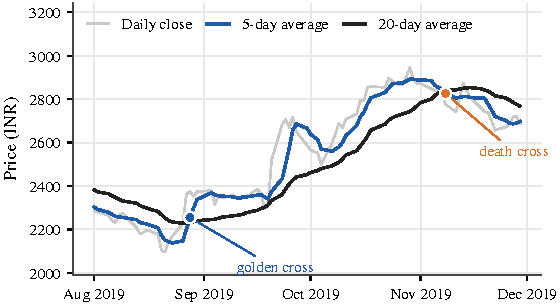
\includegraphics[width=0.66\textwidth]{figures/cross.pdf}
\caption{A golden cross and a death cross in Britannia Industries; the time frame is from August to
November 2019. The golden cross is the day the 5-day moving average of the closing price
rises above the 20-day average; the death cross is the day the 5-day moving average falls back below the 20-day.
The ratio of the two averages, one of the four features used in the first part of this study, is above one
between the two crossings and below one outside them.}
\label{fig:cross}
\end{figure}

The academic evidence on these rules is mixed and has weakened over time.
\citet{lo2000} put the visual patterns of technical analysis on a statistical
footing and find that several carry incremental information about returns.
\citet{brock1992} found that moving-average and trading-range rules applied to the
Dow Jones Industrial Average from 1897 to 1986 produced returns that standard null
models of prices could not explain; \citet{sullivan1999} re-examined the same
universe of rules with a bootstrap that corrects for data snooping and found that
the best rule's performance did not carry over into the following decade. In their
survey of 95 modern studies, \citet{park2007} report that most find profits until
the early 1990s, but that many are affected by data snooping, ex post selection of
rules and difficulties in measuring risk and transaction costs. \citet{welch2008}
show that most variables proposed as predictors of equity returns fail once they
are evaluated on data not used to select them.

A separate section of the literature uses past prices to compare stocks with each other rather
than to forecast one stock through time. \citet{jegadeesh1993} show that stocks
with high returns over the previous three to twelve months go on to outperform
those with low returns over the following months. \citet{george2004} find that a
stock's closeness to its 52-week high explains much of that momentum effect, \citet{han2016}
build a trend factor from moving averages of several lengths, and
\citet{carhart1997} adds momentum to the factors used to explain fund returns.
\citet{agarwalla2013} construct the same factors for Indian equities.

This paper asks a similar question. The first part of the study asks it in its narrow form: given a
stock's recent price history, summarised by four moving-average features, does a
linear model forecast the next day's return better than benchmarks that use no
model? The second part asks it in the form the momentum literature uses: ranked against
each other once a month on price signals, do the highest-ranked stocks earn more
than the rest, after the costs of trading them? Testing the second form exposed a
problem with the data. The universe of stocks was today's list of
large stocks, so every company in it had survived to today, and a backtest on
survivors overstates returns \citep{brown1992}. The final part of the study rebuilds the universe from
the exchange's own records, which include the companies that later failed, and
reruns the same strategy without changing it.

The first answer came back with negative returns. Across \NStocks{} stocks the mean out-of-sample $R^2$
is \RsqMean{} and mean directional accuracy is \AccMean, and no stock's accuracy is
significantly above 50\%. The second answer gave better results; on today's Nifty 500 the strategy returns \SurvCagrFull{} a
year from March 2009 to June 2026. Survivorship accounts for about \BiasRounded{}
percentage points of both the strategy's and the benchmark's return. On the
corrected data the strategy returns \PitCagrFull{} a year, against \PitEwCagrFull{}
for an equal-weighted portfolio of the same stocks and \PitNiftyCagrFull{} for the
Nifty 500, and in the holdout, which was run once after the model was altered, it
beats that benchmark by \PitActiveHold{} a year ($t = \PitActiveTHold$). Its excess
return is the momentum premium: once a momentum factor is controlled for, nothing
is left.

The paper provides three insights. It provides out-of-sample evidence that daily
moving-average features carry no useful information for a recent sample of Indian
stocks. It tests a documented premium as a long-only strategy an investor could
hold, taking into account Indian transaction costs and a one-day execution lag. And it also measures survivorship bias in
an Indian backtest directly, by running one strategy on three universes: the bias
inflated absolute returns by about \BiasRounded{} points a year, while the strategy's return
relative to its benchmark stayed similar, with a difference of a few basis points.

I came to this question through an equity research internship at BugleRock
Capital, where the contrast between fundamental analysis and technical trading came
up repeatedly. Intrigued by how technical analysis worked, I felt that testing the most popular technical signal on data
it had not seen was the most direct way to find out how much the evidence supports it. 

Section~\ref{sec:partone} presents Part~I. Section~\ref{sec:parttwo} sets out the
design of the monthly strategy and its results on today's Nifty 500, and
Section~\ref{sec:partthree} rebuilds the universe and reruns it.
Section~\ref{sec:weak} reports robustness checks and weak points,
Section~\ref{sec:discussion} discusses the findings and Section~\ref{sec:limits}
their limitations. Section~\ref{sec:conclusion} concludes.

% ======================================================================
\section{Part I: A next-day forecast}\label{sec:partone}

\subsection{Data and design}

The universe consists of \NUniverse{} companies listed on the National Stock
Exchange of India, chosen to span large, mid and small capitalisation. Daily closing
prices from 1~June 2019 to 30~June 2026 were downloaded from Yahoo Finance. Two
stocks returned no usable history and are excluded, leaving \NStocks.

Let $P_t$ denote a stock's adjusted close on day $t$. The four features use closes
up to and including day $t$:
\begin{equation}\label{eq:features}
  \mathit{ma5}_t = \frac{1}{5}\sum_{i=0}^{4} P_{t-i}, \qquad
  \mathit{ma20}_t = \frac{1}{20}\sum_{i=0}^{19} P_{t-i}, \qquad
  r_t = \frac{P_t}{P_{t-1}} - 1, \qquad
  \mathit{ratio}_t = \frac{\mathit{ma5}_t}{\mathit{ma20}_t}.
\end{equation}
The ratio, when above one, depicts the golden-cross state and, when below one, the death-cross
state, so it expresses the crossing rule as a continuous variable. For each stock
$i$, the model
\begin{equation}\label{eq:model}
  r_{i,t+1} = \beta_{i0} + \sum_{k=1}^{4} \beta_{ik}\, \tilde x_{ik,t} + \varepsilon_{i,t+1}
\end{equation}
is estimated by ordinary least squares, where $\tilde x_{ik,t}$ is feature $k$
standardised to zero mean and unit variance \citep{pedregosa2011}. The first 80\%
of each stock's observations, June 2019 to January 2025 for a stock with a full
history, form the estimation sample, and the remaining 20\% the evaluation sample.
The split is chronological, the standardisation uses estimation-sample statistics, 
and nothing is re-estimated during the evaluation sample.

Three statistics are computed on each stock's evaluation sample of $n_i$ days. The
out-of-sample $R^2$ compares the model with a constant forecast,
\begin{equation}\label{eq:r2}
  R^2_{OS,i} = 1 - \frac{\sum_t \left(r_{i,t+1} - \hat r_{i,t+1}\right)^2}
                       {\sum_t \left(r_{i,t+1} - \bar r_i\right)^2},
\end{equation}
where $\bar r_i$ is the mean return over the evaluation sample, a stricter reference
than the estimation-sample mean of \citet{campbell2008}. Directional accuracy is the
share of days on which forecast and realised returns have the same sign, and the
\emph{edge} is the model's accuracy minus the accuracy of a rule that always predicts a rise,
which equals the share $b_i$ of up days in the evaluation sample. A forecast with no
information that predicts a rise with probability one half has expected accuracy of
50\%, so its expected edge is
\begin{equation}\label{eq:randomedge}
  \mathbb{E}\left[\mathrm{Edge}_i \mid \text{uninformative forecast}\right] = \tfrac12 - b_i ,
\end{equation}
which is positive whenever up days are in the minority. Each stock's accuracy is
tested against 50\% with an exact binomial test, corrected for testing \NStocks{}
hypotheses with the procedure of \citet{benjamini1995}, and with the test of
\citet{pesaran1992}, which allows for the base rate of up days.

\subsection{Results}

Table~\ref{tab:summary} summarises the evaluation. The mean out-of-sample $R^2$ is
\RsqMean{} and the median \RsqMedian. \NRsqNeg{} of \NStocks{} $R^2$ values are negative
and the remaining \NRsqPos{} positive $R^2$ values are all small (Figure~\ref{fig:fit}, Panel A). A
negative $R^2$ basically means that the fitted model forecasts next-day returns less
accurately than a constant, which is the outcome expected when the regressors carry
no information: the coefficients are fitted to noise in the estimation sample, and
the noise does not recur.

\begin{table}[!htbp]
\centering
\caption{Part I: Out-of-sample performance across \NStocks{} stocks}
\label{tab:summary}
\small
\begin{tabular}{@{}lr@{}}
\toprule
\multicolumn{2}{@{}l}{\textit{Panel A. Fit of the return forecast}} \\
\quad Mean $R^2_{OS}$ & \ensuremath{-0.0155} \\
\quad Median $R^2_{OS}$ & \ensuremath{-0.0090} \\
\quad Range & \ensuremath{-0.130} to \ensuremath{+0.042} \\
\quad Stocks with $R^2_{OS} > 0$ & 17 of 98 \\
\addlinespace
\multicolumn{2}{@{}l}{\textit{Panel B. Direction of the forecast}} \\
\quad Mean directional accuracy & 49.6\% \\
\quad Range of directional accuracy & 41.3\% to 55.3\% \\
\quad Mean share of up days (always-up benchmark) & 47.8\% \\
\quad Mean edge over always-up (pp) & \ensuremath{+1.85} \\
\quad Expected edge of an uninformative forecast (pp) & \ensuremath{+2.22} \\
\quad Stocks with a positive edge & 68 of 98 \\
\addlinespace
\multicolumn{2}{@{}l}{\textit{Panel C. Per-stock inference, 5\% level}} \\
\quad Accuracy significantly above 50\% (binomial) & 0 \\
\quad Accuracy significantly below 50\% (binomial) & 7 \\
\quad Significant after Benjamini-Hochberg & 0 \\
\quad Significant Pesaran-Timmermann statistic & 5 \\
\addlinespace
\multicolumn{2}{@{}l}{\textit{Panel D. The moving-average ratio}} \\
\quad Stocks where \texttt{ma\_ratio} has the largest coefficient & 0 of 98 \\
\quad Positive coefficient & 61 of 98 \\
\quad Mean absolute coefficient & 0.0016 \\
\bottomrule
\end{tabular}

\begin{tablenote}
Statistics are computed on each stock's evaluation sample and averaged across
stocks where stated. $R^2_{OS}$ is defined in equation~\eqref{eq:r2}. The
always-up benchmark's accuracy equals the share of up days. The expected edge of an
uninformative forecast is $\tfrac12 - b_i$ from equation~\eqref{eq:randomedge},
averaged across stocks. Panel C counts stocks significant in two-sided tests at the
5\% level; the Pesaran-Timmermann statistic is defined for \NPTDefined{} stocks.
pp denotes percentage points.
\end{tablenote}
\end{table}

\begin{figure}[!htbp]
\centering
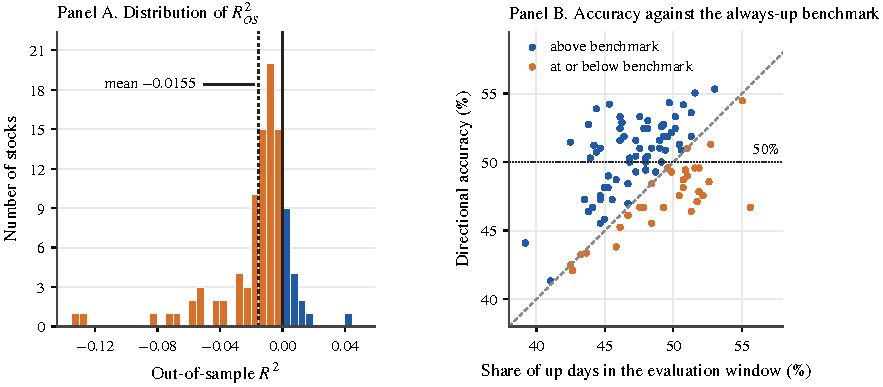
\includegraphics[width=\textwidth]{figures/fit_and_direction.pdf}
\caption{Part I: Explained variance and directional accuracy. Panel A shows the
distribution of $R^2_{OS}$ across stocks, with values above zero in blue; the solid
line marks zero and the dashed line the mean. Panel B plots each stock's
directional accuracy against the share of up days in its evaluation window, which
represents the accuracy of the always-up rule. Points above the dashed 45-degree line beat
that rule; the dotted line marks 50\%.}
\label{fig:fit}
\end{figure}

Mean directional accuracy is \AccMean. The model beats the always-up rule for
\NEdgePos{} of \NStocks{} stocks, by \EdgeMean{} percentage points on average, but
this is not necessarily a positive result, because the benchmark is naive: it uses no model. Over the evaluation
window, the median stock's price changed by \MedianTestChange, so up days were in the
minority for \NWeakBench{} stocks and the always-up rule averaged only \UpMean. By
equation~\eqref{eq:randomedge}, a forecast with no information would have beaten it
by \RandomEdge{} points on average.
Figure~\ref{fig:edge} makes the comparison stock by stock: the model's edge tracks
the edge an uninformative forecast would have earned, with a correlation of
\EdgeBenchCorr{} across stocks.

\begin{figure}[!htbp]
\centering
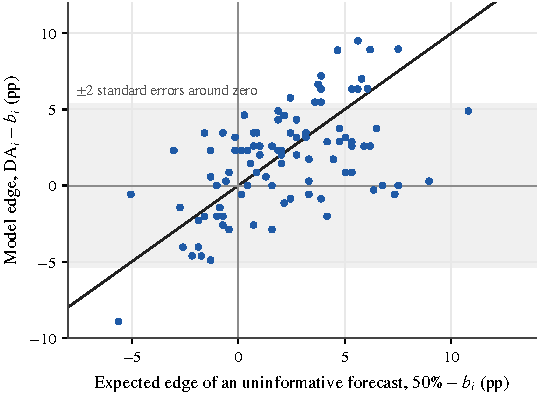
\includegraphics[width=0.62\textwidth]{figures/edge_vs_random.pdf}
\caption{Part I: The model's edge against the edge of an uninformative forecast.
Each point is a stock. The horizontal axis is $\tfrac12 - b_i$, the expected edge
over the always-up rule of a forecast that predicts a rise with probability one
half; the vertical axis is the model's realised edge. The solid line is the
45-degree line on which the two are equal. The shaded band is two standard errors
of a single stock's accuracy around zero.}
\label{fig:edge}
\end{figure}

In the binomial tests, no stock is significantly above 50\% and \NSigBelow{} are
significantly below, about the number expected by chance, and none of them survives
the correction for multiple testing. The Pesaran-Timmermann statistic is significant
at 5\% for \NPTSigPos{} of \NPTDefined{} stocks and for none after the same
correction. The moving-average ratio, the feature that encodes the crossing rule,
has the largest standardised coefficient for none of the \NStocks{} stocks.

\subsection{Why the target is a return}\label{sec:levels}

A natural alternative design forecasts the next day's price rather than its
return. For example, for Reliance Industries, a model with the same features fitted to the next
day's close attains an $R^2$ of \RelPriceRsq{} over the \RelTestDays{} evaluation
days (Table~\ref{tab:reliance}), the kind of figure that suggests a strong model.
The random walk, which forecasts tomorrow's close as today's, attains \RelNaiveRsq{}
without estimating anything, with a mean absolute error \RelMAEcut{} lower. The
reason is in the denominator of $R^2$. Over the evaluation sample the close had a
standard deviation of \rupee\RelCloseSD, while a typical daily move was
\rupee\RelRWRMSE, so any forecast close to the previous close explains most of the
variance of the level, whether or not it anticipates the change.

\begin{table}[!htbp]
\centering
\caption{Part I, Reliance Industries: Level and return forecasts over the evaluation sample}
\label{tab:reliance}
\small
\begin{tabular}{@{}lrrr@{}}
\toprule
 & Price model & Random walk & Return model \\
\midrule
MAE & \rupee18.23 & \rupee13.26 & 0.0097 \\
RMSE & \rupee23.70 & \rupee18.08 & 0.0133 \\
$R^2$ against the test mean & 0.9363 & 0.9629 & $-$0.0080 \\
Directional accuracy (\%) & 47.0 & 51.6 & 51.0 \\
\bottomrule
\end{tabular}

\begin{tablenote}
The price model and the return model use the same four features, the same split
and the same estimator; only the target differs. The random walk forecasts
tomorrow's close as today's close; because it never forecasts a rise, its
directional accuracy is the share of days on which the price did not rise. MAE and
RMSE for the first two columns are in rupees; the return model's errors are
fractions of the price.
\end{tablenote}
\end{table}

The last row of Table~\ref{tab:reliance} scores direction, and there the high $R^2$
counts for nothing: the price model calls the next day's move correctly on
\RelPriceDir{} of days, worse than the probability of heads on a coin flip. Figure~\ref{fig:parity} plots each
forecast against the outcome. The level forecasts lie along the diagonal because
prices change little from one day to the next, while the return forecasts form a
narrow vertical band within \RelPredBand{} of zero. For an autocorrelated series
such as a price level, the right reference for $R^2$ is the random walk, not the
sample mean.

\begin{figure}[!htbp]
\centering
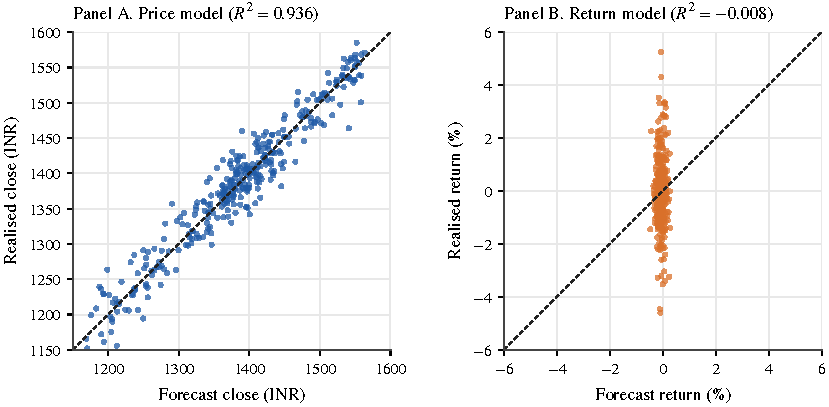
\includegraphics[width=\textwidth]{figures/reliance_parity.pdf}
\caption{Part I: Forecast against realised values for Reliance Industries over the
same \RelTestDays{} evaluation days. Panel A is the price model and Panel B the
return model; the dashed line marks perfect forecasts.}
\label{fig:parity}
\end{figure}

\subsection{What the null result suggested}

The results are consistent with the weak form of the efficient market hypothesis
\citep{fama1970} at the daily horizon, but the design limited what they could show.
Each stock was forecast on its own history, one day ahead, with no portfolio and no
costs, and about 345 evaluation days per stock gave too little power to detect an
effect of one or two percentage points of accuracy. The literature on price signals
that do carry information measures them differently: across stocks rather than
through time, over months rather than days, and as the return of a portfolio rather
than the accuracy of a forecast \citep{jegadeesh1993}. Part~II of this study tests price signals
in that form.

% ======================================================================
\section{Part II: A monthly strategy}\label{sec:parttwo}

\subsection{Universe and data}

The universe is the Nifty 500, as it stood when the data were downloaded in October
2026, \NSurvivorUniverse{} stocks with a price history, with daily closes and volumes
from January 2005 to June 2026 from Yahoo Finance. The adjusted closes include
dividends.\footnote{Part~I's paper stated that returns excluded dividends. Comparing
Yahoo's adjusted and unadjusted closes around ITC's ex-dividend dates shows that the
adjusted series includes them.} I cleaned the prices before any signal was computed:
one-day spikes that reverse within five sessions were removed as bad ticks, a
stock's history restarts after a suspension of 60 sessions or more, and splits,
bonuses and demergers that Yahoo leaves in its adjusted series were repaired.

At each month-end a stock is eligible if it has 252 sessions of history, traded on
at least \MinTradedPct{} of the last 252 sessions, and is not among the least liquid
\LiqDropPct{} of the remaining stocks by six-month median traded value. Each check
uses data up to that month-end only.

\subsection{Signals and how they were chosen}

I fixed a list of \NCandidates{} candidate signals
(Table~\ref{tab:signals}). They are price-based signals with a published rationale:
12-1 momentum \citep{jegadeesh1993}, closeness to the 52-week high
\citep{george2004}, the ratio of a moving average to the price at five horizons,
which generalises Part~I's feature and follows \citet{han2016}, low volatility,
one-month reversal and a volume shock. On each month-end every signal is winsorised
at the 1st and 99th percentiles across eligible stocks and standardised to a
$z$-score.

\begin{table}[!htbp]
\centering
\caption{The candidate signals and the selection rule}
\label{tab:signals}
\small
\begin{tabular}{@{}llrrl@{}}
\toprule
Signal & Definition & Mean IC & $t$ & Selected \\
\midrule
12-1 momentum & $P_{t-21}/P_{t-252} - 1$ & $+$0.044 & $+$2.55 & yes, $+$ \\
Close / 52-week high & $P_t / \max_{252} P$ & $+$0.044 & $+$2.39 & yes, $+$ \\
5-day trend & $\mathrm{MA}_5/P_t$ & $+$0.022 & $+$1.90 & no \\
20-day trend & $\mathrm{MA}_{20}/P_t$ & $+$0.006 & $+$0.56 & no \\
50-day trend & $\mathrm{MA}_{50}/P_t$ & $-$0.007 & $-$0.52 & no \\
100-day trend & $\mathrm{MA}_{100}/P_t$ & $-$0.027 & $-$1.79 & no \\
200-day trend & $\mathrm{MA}_{200}/P_t$ & $-$0.037 & $-$2.18 & yes, $-$ \\
Low volatility & $-\sigma_{252}$ & $+$0.026 & $+$1.49 & no \\
1-month reversal & $-(P_t/P_{t-21} - 1)$ & 0.000 & $-$0.02 & no \\
Volume shock & $\log(\overline{V}_{20}/\overline{V}_{252})$ & $+$0.021 & $+$2.01 & yes, $+$ \\
\bottomrule
\end{tabular}

\begin{tablenote}
$P_t$ is the close at month-end $t$, with lags in trading sessions;
$\mathrm{MA}_L$ is the $L$-session moving average, $\sigma_{252}$ the volatility of
daily returns over 252 sessions and $\overline V_n$ the mean daily traded value over
$n$ sessions. The information coefficient (IC) is the rank correlation across
eligible stocks between the signal and the next month's return; $t$ is the
Newey-West $t$-statistic of its mean with \NWLags{} lags, on signal dates from
January 2006 to October 2018. A signal is selected if $|t| \geq \TThreshold$, with
the sign of its mean IC. The last column applies the same rule to the
survivorship-free data of Section~\ref{sec:partthree}; it is reported only.
\end{tablenote}
\end{table}

The selection rule was fixed before the data were examined: a signal enters the
strategy if the mean of its monthly rank information coefficient (IC) on the
development period has a Newey-West $t$-statistic \citep{newey1987} of at least
\TThreshold{} in absolute value, with the sign of that mean. Four signals passed:
12-1 momentum ($t = \DevTMom$), closeness to the 52-week high ($t = \DevTHigh$), the
volume shock ($t = \DevTVol$) and the 200-day trend ($t = \DevTTrend$), which enters
with a negative sign, so a close above its 200-day average scores well
(Figure~\ref{fig:signals}, Panel A).

\begin{figure}[!htbp]
\centering
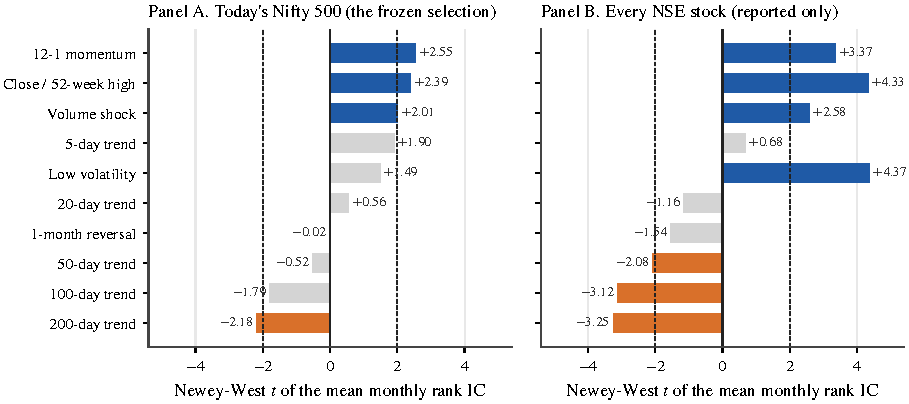
\includegraphics[width=\textwidth]{figures/strategy_signals.pdf}
\caption{Signal selection on the development period. Each bar is the Newey-West
$t$-statistic of a signal's mean monthly rank IC. Signals beyond the dashed lines at
$\pm\TThreshold$ are selected, in blue with a positive sign and orange with a
negative one. Panel A is the selection that fixed the strategy. Panel B applies the
same rule to the survivorship-free data built in Section~\ref{sec:partthree}; it
selects \NSelectedNse{} signals, including all four of Panel A, and is reported only.}
\label{fig:signals}
\end{figure}

\subsection{Portfolio, costs and timing}

The score of a stock is the average of its four selected $z$-scores, each with the
sign of its IC. At each month-end the strategy buys the top fifth of eligible stocks
by score in equal weights and holds them, with weights drifting with prices, until
the next month-end. It is long only, since an investor cannot hold a short
position overnight in the Indian cash market. The signal uses the month-end close
and the trade is made at the close of the next session, so the price that produced a
signal is never the price paid.

Each trade is charged the delivery costs in force on the NSE since October 2024:
securities transaction tax of \CostSTT{} on both purchases and sales, stamp duty of
\CostStamp{} on purchases, exchange and SEBI fees with goods and services tax on
them, no brokerage, and a bid-ask spread of \SpreadLow, \SpreadMid{} or
\SpreadHigh{} basis points for the most, middle and least liquid third of the
universe. The benchmark is an equal-weighted portfolio of every eligible stock (EW),
rebalanced on the same dates and charged the same costs. It shares the strategy's
universe, so any bias in the universe affects both, and the comparison between them
is the test of the signals.

\subsection{Protocol}

The development period runs from March 2009 to December 2018 and the holdout from
January 2019 to June 2026. Every choice described above, including the cost
schedule and the list of variants to report, was committed to a GitHub repository before
any backtest was run, and while the specification was being fixed the code that
loads prices stopped at December 2018. One choice changed on development data. At first,
a walk-forward \citet{fama1973} regression of returns on
the four signals was the primary model; on the development period its forecasts had a
negative rank IC, because slopes estimated through the 2008--09 crash put large
offsetting weights on correlated signals. I replaced it with the equal-weighted
score before the holdout was opened. The
holdout was then run once again.

\begin{figure}[!htbp]
\centering
\begin{tikzpicture}[node distance=0.32cm]
  \tikzset{box/.style={stage=2.75cm, inner sep=3pt, minimum height=1.4cm}}
  \node[box] (s1) {Specification\\ committed, prices\\ cut at Dec 2018};
  \node[box, right=of s1] (s2) {Primary model\\ chosen on\\ development data};
  \node[box, right=of s2] (s3) {Holdout\\ unlocked and\\ run once};
  \node[box, right=of s3] (s4) {NSE data rules\\ committed before\\ any backtest};
  \node[box, right=of s4] (s5) {Same strategy\\ rerun once on\\ NSE data};
  \foreach \a/\b in {s1/s2, s2/s3, s3/s4, s4/s5} \draw[flow] (\a) -- (\b);
  \node[note, above=0.12cm of s2] {Part II};
  \node[note, above=0.12cm of s4] {Part III};
  \coordinate (t0) at ($(s1.south west)+(0,-0.85)$);
  \coordinate (t1) at (s5.south east |- t0);
  \coordinate (ta) at ($(t0)!0.19!(t1)$);
  \coordinate (tb) at ($(t0)!0.65!(t1)$);
  \fill[black!8] (t0) rectangle ($(ta)+(0,0.42)$);
  \fill[accent!16] (ta) rectangle ($(tb)+(0,0.42)$);
  \fill[accentorange!22] (tb) rectangle ($(t1)+(0,0.42)$);
  \draw[rule, line width=0.5pt] (t0) rectangle ($(t1)+(0,0.42)$);
  \node[font=\footnotesize] at ($(t0)!0.5!(ta)+(0,0.21)$) {Warm-up 2005--09};
  \node[font=\footnotesize] at ($(ta)!0.5!(tb)+(0,0.21)$) {Development: Mar 2009 to Dec 2018};
  \node[font=\footnotesize] at ($(tb)!0.5!(t1)+(0,0.21)$) {Holdout: Jan 2019 to Jun 2026};
\end{tikzpicture}
\caption{The order of the work. The top row is the sequence of commits in the
repository; the bar below is the sample. Signals are selected on signal dates from
January 2006 to October 2018, whose next-month returns end within the development
period. Warm-up years provide the 252 sessions of history the signals need.}
\label{fig:protocol}
\end{figure}

\subsection{Inference}

Returns are monthly and net of costs. The return over the equal-weighted baseline strategy
(EW) is the mean monthly
difference between the strategy and EW, annualised, and its $t$-statistic uses
Newey-West standard errors with \NWLags{} lags. Alpha against EW is the annualised 
intercept of a regression of the strategy's excess return on EW's. Because
\NTrials{} configurations were evaluated, including the variants in
Section~\ref{sec:weak}, the Sharpe ratio is also reported as the deflated Sharpe
ratio of \citet{bailey2014}, the probability that it exceeds the best Sharpe ratio
expected from that many trials with no skill, and with a 95\% interval from
\NBoot{} draws of a stationary bootstrap \citep{politis1994} with a mean block of
\BootBlock{} months.

The strategy is compared with \NRandom{} random portfolios of the same size drawn from
the same eligible stocks each month, and its long-short spread with \NPlacebo{}
spreads built from scores shuffled across stocks, both before costs. The excess
returns are regressed on the market, size, value and momentum factors of
\citet{agarwalla2013}. As a test for
look-ahead, the same engine ranks stocks on their realised next-month return, which
must produce an implausible Sharpe ratio, and on scores one month stale, which must
do somewhat worse than live scores. As a test that the signals are built correctly,
the 12-1 momentum spread is compared with the published momentum factor. Unit tests
check the engine, including one that changes every price after a date and confirms
that no signal, weight or score dated before it changes.

\subsection{Results on today's Nifty 500}

Panel A of Table~\ref{tab:headline} reports the results on today's Nifty 500. The
strategy returns \SurvCagrFull{} a year over the full sample with a Sharpe ratio of
\SurvSharpeFull, against \SurvEwCagrFull{} for EW and \SurvNiftyCagrFull{} for the
Nifty 500 price index. In the holdout it beats EW by \SurvActiveHold{} a year
($t = \SurvActiveTHold$). These numbers are too high to be believed as they stand.
EW, a portfolio with no signal at all, beat the index by about ten percentage points
a year, and an equal-weighted portfolio should not outperform a cap-weighted index by
that much for seventeen years. Section~\ref{sec:partthree} shows the reason behind it.

\begin{table}[!htbp]
\centering
\caption{The strategy on two universes, net of costs}
\label{tab:headline}
\small
\begin{tabular}{@{}lrrr@{}}
\toprule
 & Development & Holdout & Full \\
 & 2009--2018 & 2019--2026 & 2009--2026 \\
\midrule
Strategy CAGR & 31.0 & 33.3 & 32.0 \\
Equal-weight universe (EW) CAGR & 26.9 & 22.7 & 25.0 \\
Nifty 500 price index CAGR & 16.1 & 13.0 & 14.8 \\
Strategy Sharpe ratio & 1.14 & 1.16 & 1.15 \\
EW Sharpe ratio & 0.81 & 0.80 & 0.81 \\
Strategy maximum drawdown & $-$27.9 & $-$36.9 & $-$36.9 \\
Return over EW, a year ($t$) & $+$2.4 (0.47) & $+$8.5 (2.67) & $+$5.0 (1.60) \\
Alpha against EW, a year ($t$) & $+$8.5 (2.73) & $+$9.9 (3.19) & $+$9.2 (4.09) \\
Deflated Sharpe ratio & 0.99 & 0.95 & 1.00 \\
Cost drag, a year & 2.6 & 2.5 & 2.5 \\
\bottomrule
\end{tabular}

\begin{tablenote}
CAGR is the compound annual growth rate. Sharpe ratios use the risk-free rate of
\citet{agarwalla2013}. EW is an equal-weighted portfolio of every eligible stock,
rebalanced monthly and charged the same costs. Panel A compares with the Nifty 500
price index, the only series Yahoo provides; Panel B with NSE Indices' total return
series. Return over EW is the annualised mean monthly difference and alpha the
annualised intercept of a regression on EW, both with Newey-West $t$-statistics. The
deflated Sharpe ratio allows for \NTrials{} configurations evaluated.
\end{tablenote}
\end{table}

% ======================================================================
\section{Part III: A survivorship-free test}\label{sec:partthree}

\subsection{The problem}

A company enters today's Nifty 500 by being among the largest listed companies now.
Companies that were large in 2010 and have since collapsed, been suspended or been
delisted are not in it, so a portfolio drawn from today's list in 2010 holds only the
stocks that went on to do well enough to remain listed and large \citep{brown1992}.
For an equal-weighted benchmark the effect is simple: its return is inflated. For a
momentum strategy it could be worse, because momentum buys past winners, and the past
winners that later failed are exactly the stocks the list leaves out.

NSE Indices publishes a Nifty500 Equal Weight index whose history it computed from
each date's actual constituents, which makes the size of the problem measurable.
From March 2009 to June 2026 the equal-weighted portfolio of today's Nifty 500
beat that index by \SurvEwGap{} a year, net of costs (Figure~\ref{fig:survivorship},
Panel A).

\subsection{Rebuilding the universe from exchange records}

NSE publishes a file for each trading session listing every security that traded,
with its close, volume and traded value. I downloaded all \NSessionsNse{} sessions
from January 2005 to June 2026, kept the equity series, excluded exchange-traded
funds, and mapped renamed symbols to their current names, using NSE's list of symbol
changes and, from 2011, matching ISINs. The panel keeps \NStocksNse{} stocks: every
equity that was among the 1,000 most traded at some month-end.
The universe is rebuilt at each month-end from what was trading then: the
\PitTopN{} most traded stocks by six-month median traded value, which is about the
size of the Nifty 500, followed by the same eligibility rules as before. That leaves
\PitUniverse{} stocks each month, and \NEverEligible{} different stocks pass through
the universe over the sample. Traded value ranks stocks by investability rather than
by market capitalisation, because a history of shares outstanding is not freely
available, and it needs no adjustment for splits.

The exchange's prices are transaction prices, with no adjustment
for corporate actions. For the period from January 2010 onward,
corporate action information was obtained from NSE's corporate action records.
Listing every unexplained one-day fall of more than 40\% in a liquid
stock found \NMissingSplits{} splits and bonuses missing from NSE's records, each of
which was verified against the company's filing. Before 2010 the records did not exist, so
capital changes are found from prices: a fall close to a standard split or bonus
ratio in a liquid stock, or a fall of more than 80\% in any stock. Both rules were
checked on 2010--2026, where NSE's records give the answer: the first flags
\SplitRuleN{} moves of which \SplitRuleHit{} were recorded corporate actions, the
second \HugeRuleN{} of which \HugeRuleHit{} were. Large falls that fit neither rule are
kept as real returns.


A stock that stops trading needs a final return. A merger or a voluntary delisting
pays its holders the acquirer's shares or an exit offer, so its final return is set
to zero. A compulsory delisting, a liquidation, or an exit after the stock had been
moved to NSE's trade-for-trade segment or lost half its price in its last year is
treated as distress and given a final return of \DistressReturn, the convention of
\citet{shumway1997}, with 0\% and $-$100\% reported as bounds. A suspension of 60
sessions or more that ends in resumed trading books the actual price change across
the gap.

Two comparisons assess the rebuilt return series. For stock-months covered by both
sources from 2010 onward, the rebuilt monthly return is within one percentage point
of Yahoo's in \YahooAgree{} of the \YahooMonths{} observations. Before 2010, the
share is \YahooAgreeEarly; this comparison is less direct because NSE's records do
not include dividends for those years. The rebuilt universe's equal-weighted
portfolio earns \PitEwGrossCagr{} a year before costs, compared with
\IndexEwCagr{} for NSE's Nifty500 Equal Weight index. Their monthly returns have a
correlation of \PitEwGrossCorr, indicating that the portfolio generally moves with
the index. Its lower return is consistent with the conservative treatment of stock
exits and the omission of dividends where records are unavailable.

\subsection{Protocol}

The rules in this section were fixed by checking the data alone, against Yahoo,
against NSE's index and against NSE's own records, and were fixed before any
strategy return on the new data was computed. The strategy was then run once,
unchanged. Because the holdout had already been seen in Part~II, this is a
replication of the same strategy on corrected data, not a new out-of-sample test.

\subsection{Results}

Panel B of Table~\ref{tab:headline} and Figure~\ref{fig:growth} report the results.
Over the full sample the strategy returns \PitCagrFull{} a year with a Sharpe ratio
of \PitSharpeFull, against \PitEwCagrFull{} and \PitEwSharpeFull{} for EW and
\PitNiftyCagrFull{} and \PitNiftySharpeFull{} for the Nifty 500 total return index.
Its worst drawdown, \PitMaxDDFull, is shallower than EW's \PitEwMaxDDFull. Its return
over EW is \PitActiveFull{} a year ($t = \PitActiveTFull$) and its alpha against EW
\PitAlphaFull{} ($t = \PitAlphaTFull$). In the holdout the return over EW is
\PitActiveHold{} ($t = \PitActiveTHold$) and the alpha \PitAlphaHold{}
($t = \PitAlphaTHold$). The development period is weaker on its own: the return over
EW of \PitActiveDev{} has a $t$-statistic of only \PitActiveTDev, and only the alpha
($t = \PitAlphaTDev$) is significant there. The deflated Sharpe ratio is
\PitDsrFull{} for the full sample and \PitDsrHold{} for the holdout. The strategy
holds about \PitNamesFull{} stocks, replaces about \PitTurnoverFull{} of the
portfolio a year and pays \PitCostFull{} a year in costs; its return over EW falls to
zero only at \PitBreakEvenFull{} times the cost schedule.

\begin{figure}[!htbp]
\centering
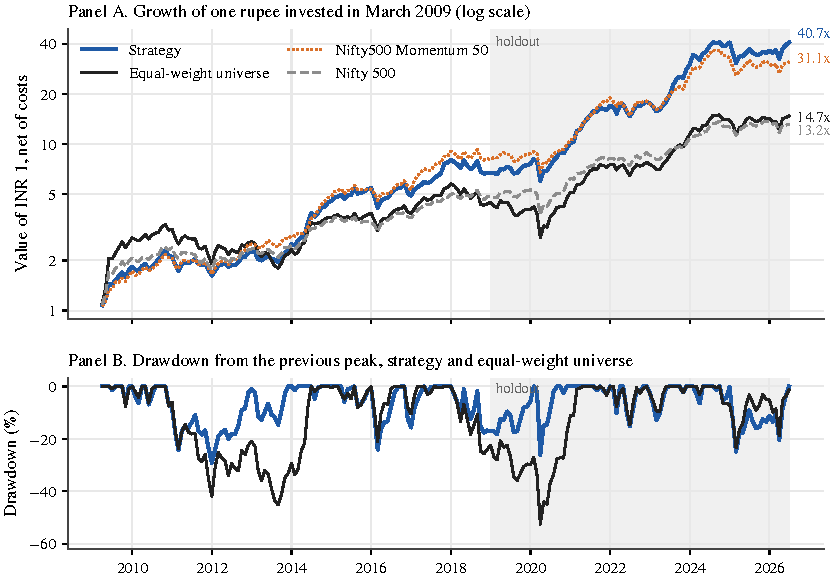
\includegraphics[width=\textwidth]{figures/strategy_growth.pdf}
\caption{The strategy on the survivorship-free universe, net of costs. Panel A shows
the value of one rupee invested in March 2009, on a logarithmic scale, with the
final multiple at the right; the shaded area is the holdout. The Nifty 500 and the
Nifty500 Momentum 50 are NSE Indices' total return series, which pay no costs.
Panel B shows the fall of the strategy and EW from their previous peaks.}
\label{fig:growth}
\end{figure}

\subsection{How much was survivorship}

Table~\ref{tab:decomposition} shows the results from running the same strategy on three universes. Moving from
Yahoo's prices to NSE's, with today's Nifty 500 names in both,
the strategy's return changes only by \BiasSource{} percentage points a year, so the data source
is not what affects the strategy. Moving from today's names to every stock that was trading at
the time lowers the strategy's return by \BiasStrategy{} points a year and EW's by
\BiasEw{} points. The bias was large, and it lifted the strategy and its benchmark by
almost exactly the same amount: the return over EW is \SurvActiveFull{},
\PitSurvActiveFull{} and \PitActiveFull{} a year on the three universes. The concern
that momentum would profit most from a universe of survivors does not show up in
these data. The likely reason appears in Section~\ref{sec:weak}: companies on their
way to failure leave the 500 most traded stocks well before they stop trading, so
the strategy rarely holds them when they do.

\begin{table}[!htbp]
\centering
\caption{One strategy on three universes, March 2009 to June 2026}
\label{tab:decomposition}
\small
\begin{tabular}{@{}lrrrrr@{}}
\toprule
 & \multicolumn{2}{c}{CAGR} & Return over & Four-factor alpha & EW minus \\
\cmidrule(lr){2-3}
Universe & Strategy & EW & EW ($t$) & over EW ($t$) & Nifty500 EW \\
\midrule
Today's Nifty 500, Yahoo prices & 32.0 & 25.0 & $+$5.0 (1.60) & $+$0.2 (0.11) & $+$6.4 \\
Today's Nifty 500, NSE prices & 31.7 & 24.7 & $+$5.1 (1.62) & $+$0.1 (0.04) & $+$6.1 \\
Every stock trading at the time, NSE & 23.8 & 16.8 & $+$5.2 (1.43) & $+$0.2 (0.09) & $-$1.9 \\
\bottomrule
\end{tabular}

\begin{tablenote}
All returns are net of costs and in percent a year. The four-factor alpha is the
annualised intercept of a regression of the strategy's monthly return minus EW's on
the factors of \citet{agarwalla2013}, to \FactorEnd. The last column is EW's
compound annual return minus that of NSE's Nifty500 Equal Weight total return index,
which NSE computes from each date's actual constituents.
\end{tablenote}
\end{table}

\begin{figure}[!htbp]
\centering
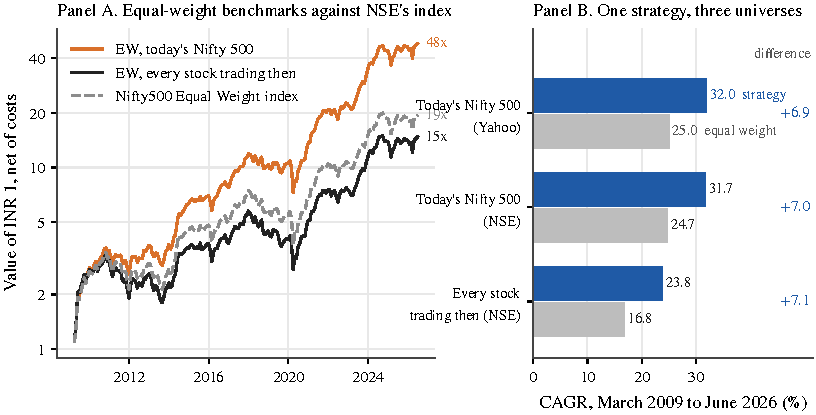
\includegraphics[width=\textwidth]{figures/survivorship.pdf}
\caption{Survivorship bias. Panel A shows the value of one rupee in the
equal-weighted portfolio of today's Nifty 500, in the equal-weighted portfolio of
every stock trading at the time, and in NSE's Nifty500 Equal Weight index, which is
built from each date's actual constituents. Panel B shows the compound annual return
of the strategy and of its equal-weighted benchmark on each of the three universes,
and the difference between them.}
\label{fig:survivorship}
\end{figure}

\subsection{Skill, luck or leakage}

Table~\ref{tab:skill} reports the checks of Section~\ref{sec:parttwo} on the
survivorship-free data. The score's mean monthly rank IC is \PitIcFull{} over the
full sample ($t = \PitIcTFull$) and \PitIcHold{} in the holdout ($t = \PitIcTHold$).
Before costs, the strategy's Sharpe ratio of \PitGrossSharpeFull{} exceeds that of
all \NRandom{} random portfolios, whose 95th percentile is \PitRandomTopFull, and its
long-short spread beats \PitPlaceboPctFull{} of the shuffled spreads. Ranking on the
realised return produces a Sharpe ratio of \PitCanaryFull, as it should, and scores
one month stale do slightly worse than live ones, \PitStaleFull{} against
\PitSharpeFull, so information reaches the portfolio at the time it should and not
before. The 12-1 momentum spread built here has a correlation of \PitWmlCorr{} with
the momentum factor of \citet{agarwalla2013}. Returns rise steadily across the five
quintiles of the score (Figure~\ref{fig:skill}).

\begin{table}[!htbp]
\centering
\caption{Skill, luck and leakage on the survivorship-free universe}
\label{tab:skill}
\small
\begin{tabular}{@{}lrrr@{}}
\toprule
 & Development & Holdout & Full \\
\midrule
Mean monthly rank IC of the score ($t$) & $+$0.068 (3.46) & $+$0.042 (2.13) & $+$0.055 (3.85) \\
Random portfolios beaten, of 1,000 & 100\% & 100\% & 100\% \\
Strategy Sharpe ratio before costs & 0.81 & 1.04 & 0.92 \\
95th percentile of random Sharpe ratios & 0.51 & 0.69 & 0.56 \\
Placebo spreads beaten, of 500 & 99.2 & 99.6 & 100.0 \\
Sharpe ratio ranking on the realised return & 4.9 & 5.9 & 5.2 \\
Sharpe ratio with scores one month stale & 0.64 & 0.85 & 0.74 \\
\bottomrule
\end{tabular}

\begin{tablenote}
The rank IC is the monthly Spearman correlation across eligible stocks between the
score and the next month's return, with a Newey-West $t$-statistic. Random portfolios
hold the same number of stocks, drawn at random from the eligible stocks each month;
placebo spreads use the strategy's scores shuffled across stocks. Both are before
costs. The last two rows are the leak checks: the same engine ranking stocks on their
realised next-month return, and on scores one month old, net of costs.
\end{tablenote}
\end{table}

\begin{figure}[!htbp]
\centering
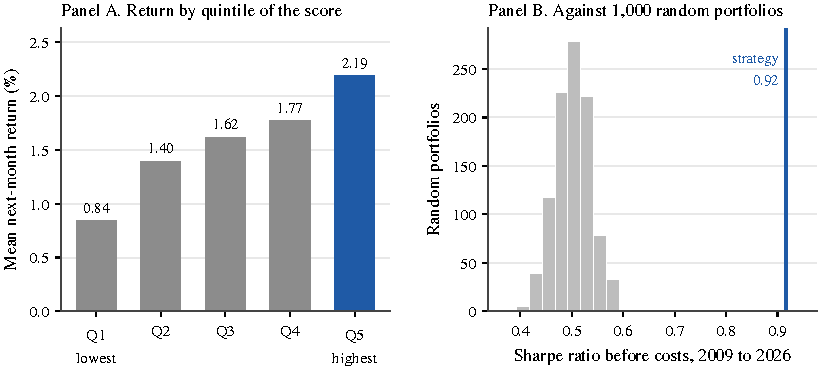
\includegraphics[width=\textwidth]{figures/strategy_skill.pdf}
\caption{Panel A shows the mean next-month return of each quintile of the score,
equal-weighted and before costs, March 2009 to June 2026; the strategy holds the top
quintile. Panel B shows the Sharpe ratios of \NRandom{} random portfolios of the same
size, before costs, and the strategy's.}
\label{fig:skill}
\end{figure}

\subsection{What the strategy earns}

Table~\ref{tab:factors} regresses the excess returns on the four factors of
\citet{agarwalla2013}. The strategy's return over EW loads on momentum with a
coefficient of \PitWml{} and leaves an alpha of \PitFactorAlpha{} a year
($t = \PitFactorAlphaT$). The edge over the benchmark is the momentum premium. The
study does not find a new anomaly; it shows that a documented one survives Indian
trading costs, a one-day execution lag and a correction for survivorship, in a form
that a long-only investor can hold.

\begin{table}[!htbp]
\centering
\caption{Four-factor attribution on the survivorship-free universe}
\label{tab:factors}
\small
\begin{tabular}{@{}lrrrrrr@{}}
\toprule
 & Alpha, a year ($t$) & Market & Size & Value & Momentum ($t$) & $R^2$ \\
\midrule
Strategy & $-$1.1 ($-$0.47) & $+$1.04 & $+$0.39 & $+$0.28 & $+$0.39 (8.5) & 0.88 \\
Equal-weight universe & $+$0.3 (0.25) & $+$1.12 & $+$0.34 & $+$0.21 & $-$0.17 ($-$6.4) & 0.97 \\
Strategy minus EW & $+$0.2 (0.09) & $-$0.04 & $+$0.05 & $+$0.04 & $+$0.52 (14.2) & 0.70 \\
\bottomrule
\end{tabular}

\begin{tablenote}
Monthly returns from March 2009 to \FactorEnd, regressed on the market, size, value
and momentum factors of \citet{agarwalla2013}. The strategy and EW are in excess of
the risk-free rate; the third row is the difference between them. Alphas are
annualised; $t$-statistics use Newey-West standard errors.
\end{tablenote}
\end{table}

NSE's own momentum index puts the result in proportion. The Nifty500 Momentum 50,
which holds the 50 stocks with the strongest risk-adjusted momentum and weights them
by momentum and size, returns \PitMomCagrFull{} a year over the same period with a
Sharpe ratio of \PitMomSharpeFull{} (Table~\ref{tab:headline}). The strategy returns
more, \PitCagrFull, with the same risk-adjusted return, \PitSharpeFull. It lagged the
index in the development period and led it in the holdout. The index pays no trading
costs, and its history before its launch in 2024 was computed by NSE with a method
chosen in 2024. The fair summary is that the strategy captures the momentum premium
about as well as a published momentum index, not better.

% ======================================================================
\section{Robustness and weak points}\label{sec:weak}

Table~\ref{tab:robustness} reports variants of the strategy, each changing one
setting. None was used to choose the primary strategy.

\begin{table}[!htbp]
\centering
\caption{Variants of the strategy on the survivorship-free universe, net of costs}
\label{tab:robustness}
\small
\begin{tabular}{@{}lrrrr@{}}
\toprule
 & \multicolumn{3}{c}{Full sample} & Holdout \\
\cmidrule(lr){2-4}\cmidrule(l){5-5}
Variant & CAGR & Sharpe & Over EW ($t$) & Over EW ($t$) \\
\midrule
Primary: composite, top quintile & 23.8 & 0.80 & $+$5.2 (1.43) & $+$8.3 (2.39) \\
Rank buffer (hold until a name leaves the top 30\%) & 25.3 & 0.85 & $+$6.4 (1.83) & $+$8.5 (2.56) \\
Fama-MacBeth forecast in place of the composite & 21.9 & 0.73 & $+$3.5 (1.04) & $+$8.0 (2.82) \\
Top decile & 25.4 & 0.80 & $+$6.9 (1.62) & $+$10.9 (2.48) \\
Top tercile & 22.4 & 0.77 & $+$3.8 (1.44) & $+$5.5 (2.05) \\
Momentum over 6 months & 23.2 & 0.76 & $+$4.7 (1.46) & $+$7.7 (2.43) \\
Momentum without the skipped month & 23.8 & 0.81 & $+$5.0 (1.39) & $+$8.1 (2.36) \\
Costs doubled & 20.6 & 0.68 & $+$2.5 (0.68) & $+$5.6 (1.61) \\
200 most traded stocks & 18.8 & 0.63 & $+$1.6 (0.46) & $+$5.9 (1.60) \\
1,000 most traded stocks & 28.8 & 0.93 & $+$7.5 (2.33) & $+$6.7 (2.22) \\
Distress exits at 0\% & 23.8 & 0.80 & $+$5.1 (1.43) & $+$8.3 (2.38) \\
Distress exits at $-$100\% & 23.8 & 0.80 & $+$5.2 (1.44) & $+$8.3 (2.39) \\
\bottomrule
\end{tabular}

\begin{tablenote}
Each row changes one setting of the primary strategy. The rank buffer keeps a stock
until it leaves the top 30\% of scores. The Fama-MacBeth variant weights the four
signals by the expanding mean of past cross-sectional regression slopes. The
universe-size and exit-return rows rebuild the universe or the exit returns and
rerun the strategy; they were specified before the replication was run. Return over
EW is in percent a year with a Newey-West $t$-statistic.
\end{tablenote}
\end{table}

\paragraph{The edge is outside the largest stocks.} Within the most liquid third of
the universe, the strategy's return over the same third's equal-weighted portfolio is
\TercileLiquidActive{} a year ($t = \TercileLiquidActiveT$), against
\TercileMiddleActive{} ($t = \TercileMiddleActiveT$) in the middle third and
\TercileIlliquidActive{} ($t = \TercileIlliquidActiveT$) in the least liquid third
(Figure~\ref{fig:weak}, Panel A). Restricted to the 200 most traded stocks, the return
over EW falls to \TopTwoHundredActiveFull{} ($t = \TopTwoHundredActiveTFull$), and
over a wider universe of 1,000 it rises to \TopThousandActiveFull{}
($t = \TopThousandActiveTFull$). This matches the finding of \citet{hong2000} that
momentum is stronger among smaller stocks.

\begin{figure}[!htbp]
\centering
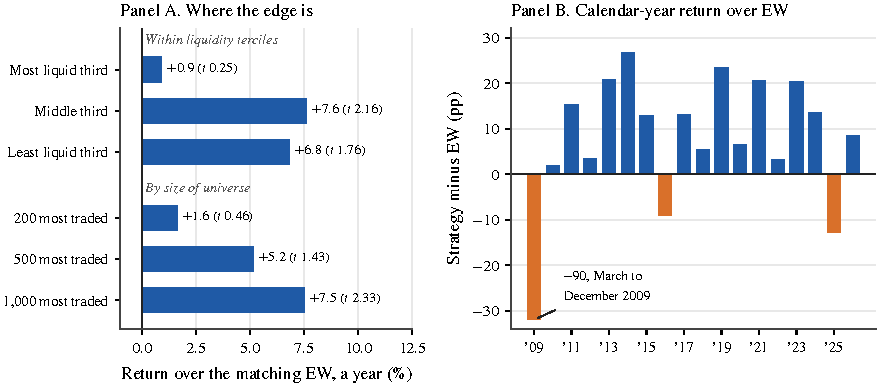
\includegraphics[width=\textwidth]{figures/strategy_weak.pdf}
\caption{Where the edge is and when it fails. Panel A shows the return over the
matching equal-weighted benchmark, a year, within each third of the universe by
liquidity and for universes of three sizes, with Newey-West $t$-statistics. Panel B
shows the strategy's calendar-year return minus EW's; 2009 runs from March and is cut
at $-$32 points, and 2026 ends in June.}
\label{fig:weak}
\end{figure}

\paragraph{Momentum crashes.} The strategy trailed EW in \YearsBehind{} of
\YearsTotal{} calendar years. The largest shortfalls came when the market turned
sharply up after a fall. From March to December 2009 the strategy returned
\YearNineStrategy{} while EW returned \YearNineEw, as the stocks that had fallen
furthest in 2008 led the recovery, the pattern \citet{daniel2016} document. In 2025
the strategy returned \YearTwentyFiveStrategy{} against \YearTwentyFiveEw. Scaling the
long-short spread by its recent volatility, as \citet{barroso2015} propose, is the
standard remedy; I report it as a variant of the spread and did not apply it to the
long-only strategy.

\paragraph{Turnover and costs.} One-way turnover is about \PitTurnoverFull{} a year,
so the strategy replaces its whole portfolio about four times a year, and costs take
\PitCostFull{} a year. It still beats EW
at twice the cost schedule (Table~\ref{tab:robustness}), but short-term capital gains
tax, which applies to positions held for less than a year and would take a large
share of the gains, is not modelled. The rank-buffer variant, which trades less,
returns \PitBufferCagr{} with a Sharpe ratio of \PitBufferSharpe, but it was not the
pre-specified primary strategy and its slightly better result is not evidence of
anything.

\paragraph{Exit returns barely matter.} Setting every distress exit to 0\% or to
$-$100\% changes the full-sample return over EW from \PitActiveFull{} to
\DistressZeroActiveFull{} and \DistressAllActiveFull. Of the \NExitsEval{} stocks that
stopped trading after March 2009, \NExitsInEw{} were in the benchmark at the
month-end before, \NExitsInEwDistress{} of them classed as distress, and
\NExitsInStrategy{} were held by the strategy, \NExitsInStrategyDistress{} as
distress. A company on its way to failure loses liquidity long before it stops
trading, and leaves the universe first.

\paragraph{The long-short spread.} The return of the top quintile minus the bottom
quintile is \PitSpreadCagr{} a year with a Sharpe ratio of \PitSpreadSharpe{} and a
maximum drawdown of \PitSpreadMaxDD. The long side does the work; the spread is
reported as a research measure, since it cannot be held in the Indian cash market.

\paragraph{Signal selection on the corrected data.} Applied to the survivorship-free
development data, the selection rule picks \NSelectedNse{} signals, the four of the
strategy and three more (Figure~\ref{fig:signals}, Panel B). The strategy keeps the
four it was fixed with. Testing the larger set would be a new search on data whose
holdout has already been seen.

% ======================================================================
\section{Discussion}\label{sec:discussion}

The two parts of the study use the same kind of information, recent prices, and
reach opposite answers. The difference lies in how the information is used. Part~I
asked whether a stock's recent prices forecast its own return tomorrow. Part~II
asked whether stocks with strong recent prices outperform stocks with weak ones over
the next month. The first is a forecast of noise-dominated daily changes, judged one
stock at a time; the second is a comparison across stocks at the horizon at which
\citet{jegadeesh1993} found momentum, and it pools the evidence across hundreds of
stocks and two hundred months. The null result of Part~I is consistent with the
weak form of the efficient market hypothesis \citep{fama1970} at the daily horizon.
The result of Part~II is consistent with a momentum premium that has persisted in
India, as the positive momentum factor of \citet{agarwalla2013} shows, and that
carries crash risk, which is one explanation for why it has not been traded away.

What the evidence supports is a long-only strategy that captures that premium net of
realistic costs, from mid-sized and less liquid stocks more than from the largest,
with a return over its benchmark that is significant in the holdout and over the
full sample by alpha, but not by the simple difference over the full sample. It does
not support a claim of returns above 30\% a year, which came from a universe of
survivors.


% ======================================================================
\section{Limitations}\label{sec:limits}

\begin{itemize}
\item \textit{The holdout was seen before Part~III.} The survivorship-free run used
  the strategy exactly as fixed in Part~II, but its holdout years were no longer
  unseen, so it is a replication rather than a second out-of-sample test.
\item \textit{Prior knowledge.} The candidate signals were chosen from a literature
  that documents momentum, including Indian evidence that covers part of the holdout
  period. The holdout was never used to fit anything, but the choice of signal family
  was not blind to how such signals have performed.
\item \textit{Data rules.} The rules that clean and adjust prices were written while
  looking at the whole sample. They were checked against independent sources and
  fixed before any strategy return was computed, but they reflect judgements: the
  exit classes are partly inferred from each stock's own record, a handful of
  pre-2010 splits in then-illiquid stocks remain unadjusted, and about one dividend
  record in ten after 2010 gives no amount.
\item \textit{Universe definition.} The universe ranks stocks by traded value rather
  than by the market capitalisation that defines the Nifty 500, and the cost schedule
  of October 2024 is applied to the whole sample.
\item \textit{Costs not modelled.} Short-term capital gains tax and the price impact
  of large orders are not deducted, and both would matter most for the less liquid
  stocks where the edge is largest.

\end{itemize}

% ======================================================================
\section{Conclusion}\label{sec:conclusion}

Four moving-average features in a linear model do not forecast the next day's
return of \NStocks{} NSE stocks better than benchmarks that use no model. The same
kind of information, when used to rank stocks against each other once a month, does
carry a premium. Holding the top fifth of a survivorship-free universe of
\PitUniverse{} stocks returned \PitCagrFull{} a year from 2009 to 2026 net of costs,
against \PitEwCagrFull{} for an equal-weighted portfolio of the same stocks, and beat
that benchmark by \PitActiveHold{} a year in a holdout that was run once. The excess
return is the momentum premium, about as large as that of NSE's momentum index and
concentrated outside the largest stocks. A universe of today's survivors would have
added about \BiasRounded{} points a year to every return in the study, which is the
main lesson for anyone backtesting on Indian equities.

Natural extensions are a universe ranked by market capitalisation, tax and
market-impact costs, signals that do not depend on price, such as earnings revisions
and delivery volumes, and a forward test that records the strategy's holdings each
month from July 2026.

% ======================================================================
\section*{Use of AI tools}

While the research question, the ideas brought in and the interpretation of the
results are my own, I used Claude Code, Anthropic's AI coding assistant, throughout this paper to learn more about computing, machine learning, and quantitative finance. 
In Part~I, it mainly acted as a tutor and wrote parts of the code under my direction. In
Parts~II and~III, Claude almost acted as a peer; it shared ideas, criticised mine and helped me find a solution to a complex problem I could not solve on my own. 
Artificial intelligence has redefined ``learning by doing'' to a whole new extent; I have learned more about computing and quantitative finance through the implementation of this project
compared to what any theory or literature on this subject would have taught me. Technical terms and concepts in the code and in finance 
that I was not familiar with, I learned through the explanations Claude provided. The process of reviewing the code, reporting the results and documenting the project alongside Claude's explanations gave me a
system where I could implement what I learned in a practical manner, which made this project more insightful.
I checked Claude's explanations against the data before relying on them. I reviewed everything it
produced and take full responsibility for the content.

\section*{Data and code availability}

{\sloppy
The project repository,
\weburl{https://github.com/arjunprashanth6129/}{price-prediction-linear-regression},
holds the prices, code and results. Part~I is in \code{scripts/ml/}, and Parts~II
and~III are in \code{scripts/strategy/}, with the exchange files of Part~III in
\code{scripts/strategy/raw/nse/}. Running \code{python paper/make\_assets.py}
re-estimates every Part~I model, checks the results against the committed output,
and regenerates all numbers, tables and figures in this paper from the committed
results of the strategy pipeline.\par}

\bibliographystyle{chicago}
\bibliography{references}

% ======================================================================
\clearpage
\appendix
\section{Part I: largest and smallest edges}

\begin{table}[h]
\centering
\caption{Stocks with the largest and smallest edge over the always-up rule}
\label{tab:extremes}
\small
\begin{tabular}{@{}rllrrrrr@{}}
\toprule
Rank & Ticker & Band & Accuracy (\%) & Up days (\%) & Edge (pp) & $R^2_{OS}$ & Binomial $p$ \\
\midrule
1 & RPOWER & Small & 53.9 & 44.4 & $+$9.5 & $-$0.072 & 0.16 \\
2 & GARFIBRES & Mid & 51.4 & 42.5 & $+$9.0 & $+$0.014 & 0.63 \\
3 & HIMATSEIDE & Small & 52.7 & 43.8 & $+$8.9 & $-$0.014 & 0.33 \\
4 & PAYTM & Large & 54.2 & 45.3 & $+$8.9 & $-$0.084 & 0.23 \\
5 & CHOLAFIN & Large & 53.3 & 46.1 & $+$7.2 & $-$0.005 & 0.24 \\
6 & GREENPANEL & Small & 51.2 & 44.2 & $+$7.0 & $+$0.008 & 0.70 \\
7 & SUPRAJIT & Small & 52.9 & 46.2 & $+$6.6 & $+$0.014 & 0.31 \\
8 & BALKRISIND & Large & 50.3 & 43.9 & $+$6.4 & $-$0.002 & 0.96 \\
\addlinespace
\multicolumn{8}{@{}c}{\textit{\dots}} \\
\addlinespace
91 & KARURVYSYA & Small & 47.6 & 50.4 & $-$2.9 & $-$0.054 & 0.39 \\
92 & HAVELLS & Large & 45.5 & 48.4 & $-$2.9 & $-$0.011 & 0.11 \\
93 & DRREDDY & Large & 47.8 & 51.9 & $-$4.0 & $-$0.006 & 0.45 \\
94 & NAVINFLUOR & Mid & 48.6 & 52.6 & $-$4.0 & $-$0.059 & 0.63 \\
95 & FEDERALBNK & Large & 47.6 & 52.2 & $-$4.6 & $-$0.025 & 0.39 \\
96 & ALKEM & Large & 47.1 & 51.7 & $-$4.6 & $-$0.012 & 0.31 \\
97 & BAJAJCON & Small & 46.4 & 51.3 & $-$4.9 & $-$0.068 & 0.20 \\
98 & LAURUSLABS & Large & 46.7 & 55.6 & $-$8.9 & $-$0.130 & 0.24 \\
\bottomrule
\end{tabular}

\begin{tablenote}
Stocks ranked by edge, the model's directional accuracy minus the share of up days
in the evaluation window, in percentage points. The binomial $p$-value tests
accuracy against 50\% and is not adjusted for multiple testing. Full results for
all \NStocks{} stocks are in \code{results/per-stock.csv} in the repository.
\end{tablenote}
\end{table}

\end{document}
